\documentclass[runningheads,a4paper]{llncs}

\usepackage{amssymb}
\setcounter{tocdepth}{3}
\usepackage{graphicx}
\usepackage{wrapfig}

\usepackage{url}
\usepackage{algpseudocode}
\usepackage{algorithm}
\usepackage{algorithmicx}



\urldef{\mailsa}\path|gorohov.art@gmail.com|    
\newcommand{\keywords}[1]{\par\addvspace\baselineskip
\noindent\keywordname\enspace\ignorespaces#1}

%To economize paper
%\textwidth=190mm
%\textheight=250mm
%\topmargin=-20mm
%\oddsidemargin=-15mm
%\evensidemargin=-15mm


\begin{document}

\algnewcommand\algorithmicswitch{\textbf{switch}}
\algnewcommand\algorithmiccase{\textbf{case}}
\algnewcommand\algorithmicassert{\texttt{assert}}
\algnewcommand\Assert[1]{\State \algorithmicassert(#1)}
% New "environments"
\algdef{SE}[SWITCH]{Switch}{EndSwitch}[1]{\algorithmicswitch\ #1\ \algorithmicdo}{\algorithmicend\ \algorithmicswitch}
\algdef{SE}[CASE]{Case}{EndCase}[1]{\algorithmiccase\ #1}{\algorithmicend\ \algorithmiccase}

\algtext*{EndSwitch}
\algtext*{EndCase}
\algtext*{EndWhile}% Remove "end while" text
\algtext*{EndIf}% Remove "end if" text
\algtext*{EndFor}% Remove "end for" text
\algtext*{EndFunction}% Remove "end function" text

\newtheorem{mydef}{Definition}

\mainmatter  % start of an individual contribution

% first the title is needed
\title{EBNF in GLL}

% a short form should be given in case it is too long for the running head
\titlerunning{EBNF in GLL}

\author{Artem Gorokhov}
\authorrunning{Artem Gorokhov}
% (feature abused for this document to repeat the title also on left hand pages)

\institute{St. Petersburg State University, Universitetsky prospekt, 28,\\
           198504 Peterhof, St. Petersburg, Russia\\
\mailsa}

\toctitle{EBNF in GLL}
\tocauthor{Artem Gorokhov}
\maketitle

%Authors are invited to submit full papers (not exceeding 12 pages) or short papers (up to 6 pages)

\begin{abstract}
% Предлагается модификация алгоритма GLL, работающая с грамматиками в форме EBNF. 
% Это приносит ошутимый прирост производительности в работе с некоторыми грамматиками языков программирования.


%At least 70 and at most 150 words.
Parsing is important step of static program analysis. 
It allows to get structural representation of code.
Parser generators a widely used for parser creation. 
EBNF is very popular for languages syntax description.
But transformation to more simple form (BNF, CNF) is required for popular tools.
There are number of works on EBNF processing without transformation.
But problems.
Generalized LL, arbitrary grammars in $O(n^s)$, factorization can increase performance...
Factorization can be improved.
We propose modification of GLL which can handle arbitrary grammar in EBNF without transformations...
performance improvements, .....

\keywords{Parsing, GLL, EBNF}
\end{abstract}


\section{Introduction}%--------------------------------------------------------------------------------------------------------------------------------------------

Static program analysis usually performed over structural representation of code and parsing is a classical way to get such representation.
Parser generators often used for parser creation automation: these tools allow to create parser from grammar of language which should be specified in appropriate format.
It allows to decrease efforts required for syntax analyzer creation and maintenance.

Extended BNF (EBNF) is a useful format of grammar specification. 
Expressive and compact description of language syntax. 
This formalism often used in documentation --- one of main source of information for parsers developers.

There are a wide range of parsing techniques and algorithms: CYK, LR(k), LALR(k), LL, etc. 
One of he most popular area is generalized parsing: technique which allows to handle ambiguous grammars. 
It is possible to simplify language description required for parser generation in case a parser generator is based on generalized algorithm.
LL family is more intuitive than LR, can provide better diagnostics, but LL(1) is not enough to process some languages: there are LR, but not LL languages.
Moreover, left and hidden left recursion in grammars is a problem. 
In order to solve these problems generalized LL (GLL) was proposed~\cite{scott2010gll}. 
This algorithm handles arbitrary context free grammar, even unambiguous and (hidden)left-recursive.
Worst-case time and space complexity of GLL is cubic in terms of input size. 
For LL grammars it demonstrates linear time and space complexity.

The problem is that classical parsing algorithms requires BNF.
It is possible to convert from EBNF to BNF but with this conversion we loose the structure of main grammar and resulting trees are for the BNF grammars.

ELL, ELR~\cite{AttributedELL,ELRR,ECFGparsing,ELLParser,ELL,ECFG,ELALR,ELRParsing} and other can process EBNF but they do not deal with ambiguities in grammars.

Factorization for GLL was introduced~\cite{scott2016structuring} but it is not full support of EBNF.

In this work we present modified generalized LL parsing algorithm which handles grammars in EBNF without transformations.
Changes are very native for GLL nature.
Proposed modifications allow to get sufficient parsing performance improvement.

This article is structured as follows.
We start from .... Extended BNF
generalized LL algorithm description.
Blah-blah


%Синтаксический анализ программ это широко известная область, ...
%Проблема в том, что грамматики, используемые в реальной жизни пишутся в форме EBNF. А GLL принимает только BNF.
%Можно проводить преобразование грамматики из EBNF к BNF, но так она разрастается, что, в некоторых случаях, замедляет процедуру разбора.
%Предлагается модификация алгоритма GLL, работающая с грамматиками в форме EBNF.



\section{EBNF processing}%--------------------------------------------------------------------------------------------------------------------------------------------

Extended Backus-Naur Form~\cite{iso} is a syntax of expressing context-free grammars. In addition to the Backus-Naur Form syntax it 
uses such constructions:
\begin{itemize}
    \item alternation $\mid$
    \item option [ ... ]
    \item repetition \{ ... \}
    \item grouping ( ... )
\end{itemize}
This form is usually used in technical documentation. While parser generators widely use Extended CFG form:
right parts of productions are regular expressions. It operates under similar constructions so EBNF can be represented in ECFG form.
In this article we will use the notation of ECFG.

An \textit{extended context-free grammar} (ECFG) is a tuple ($N$, $\Sigma$, $P$, $S$), where $N$
and $\Sigma$ are finite sets of nonterminals and terminals, $ S\in N$ is the start symbol,
and $P$ (the productions) is a map from $N$ to regular expressions over alphabet $N \cup \Sigma$.

%Regular expression syntax? Look at ``Towards a Taxonomy for ECFG and RRPG Parsing''



\section{Generalized LL Parsing}%--------------------------------------------------------------------------------------------------------------------------------------------

There are works about parsing ECFG: ELL(k)~\cite{!!!}, ELR(k)~\cite{!!!} parsers;
Early-style parsers~\cite{!!!} but none of them work with arbitrary ECFG.
Generalized algorithms (GLL and GLR) was purposed to perform syntax analysis of linear input by any context-free 
grammar, as a result we get Shared Packed Parse Forest(SPPF)~\cite{SPPF} that represents all possible derivations of input string.
Unlike the GLR, GLL algorithm~\cite{scott2010gll} is rather intuitive and allows to perform better diagnostics. 

Work of the GLL algorithm based on descriptors, it allows to handle all posible derivations.
Descriptor is a four-element tuple that can uniquely define state of parsing process. 
It is a tuple of the form $(L,i, T, S)$, where $L$ is a grammar slot ---
pointer to position in grammar of the form$(S \to \alpha \cdot \beta)$, $i$ --- a position in input,
T --- already built SPPF root, $S$ --- current Graph Structured Stack(GSS)~\cite{GSS} node.
We used efficient GSS described in~\cite{afroozeh2015faster}.
In initial state we have descriptors that describe start positions in grammar and input, dummy tree node and bottom of GSS.
On each step algorithm processes first descriptor in queue and makes some actions depending on the grammar and input.
If there are any ambiguity algorithm will queue descriptor for all cases to handle them all. 

We used table based approach which allows to generate only tables for given grammar instead of full parser code.
The idea is the same as in original article and main function uses same tree construction and stack processing functions.
Code can be found in appendix.

\subsection{Factorization}%--------------------------------------------------------------------------------------------------------------------------------------------

In order to improve performance Elizabeth Scott and Adrian Johnstone offered support of factorised grammars in GLL~\cite{scott2016structuring}. 
The idea is to automatically factorize grammars and use them for parser generation. 

Main algorithm creates and queues new descriptors depending on current parse state that we get from unqueued descriptor. 
In case descriptor was already created it does not add it to queue. For this purpose we have a set of
\textbf{all} created descriptors. Thus reducing a number of possible descriptors decreases the parse time
and required memory.

Let us spot on \textbf{slots}. Factorization decreases the number of grammar slots. 
Consider example from the paper~\cite{scott2016structuring}.
Production $P_0$ factorises to $P_0'$.
$S::= a a B c d | a a c d | a a c e | a a $
$S::= a a ( B c d | c( d | e ) | \varepsilon)$
Second is much compact and contains much less possible slots, 
so parser creates less descriptors.
It gives significant performance improvement on some grammars.

But this idea can be extended to full EBNF support.
Let us show how to do it.


\section{Extended CFG GLL Parsing}%--------------------------------------------------------------------------------------------------------------------------------------------

In this section we will show an application of Extended Context-Free Grammars(ECFG) in automatons and corresponding GLL-style parsers.

The idea of factorisation was evolved to use of automatons and their minimization.
Right parts of ECFG are regular expressions under alphabet of terminals and nonterminals.
There are some basic methods of conversion regular expressions to nondeterministic finite state automatons. 
Thus for each right-hand side of grammar productions we can build a finite state automaton, with edges tagged with 
terminals, nonterminals or $\varepsilon$-symbols. Thompson's method~\cite{Thompson:1968:PTR:363347.363387} can be used for this purpose. 
In built automatons each nonterminal edge should be complemented with name of initial state of automaton that stands 
for this nonterminal. An example of constructed automatons for grammar $\Gamma_{0}$\ref{fig:grammarG0} is given on fig.. State 0 is start state.
We call final states of automatons ``pop'' states.

Produced automatons are $\varepsilon$-NFAs under alphabet of nonterminals, terminals and $\varepsilon$ symbols.
To increase performance of parsing we can minimize the number of states in produced automatons without
loosing the structure of initial grammar.
Every automaton can be converted to determinate FA. An algorithm is described in~\cite{aho1974design}.

Decrease of the quantity of the automaton states decreases number of GLL descriptors, as it was with factorization.

Then John Hopcroft's algorithm~\cite{hopcroft1971n} can be applied to all automatons at one time. 
An algorithm is based on dividing all states on equivalent classes. Initial state of algorithm consist 
of 2 classes: first contains final states and second contains all other. For our problem we can set an 
initial state as follow: first class contains all final states of \textbf{all} automatons and second class 
contains all the other. As an algorithm result we get classes which represent new states of automaton. 
Initial state is class that contains initial state of automaton that represents productions of start nonterminal.


\subsection{Input processing}%--------------------------------------------------------------------------------------------------------------------------------------------

Slots have become automaton states. And just as we can move through grammar slots we can move through states 
in automaton. But in automaton we have nondeterministic choice because there are can be many transitions to other states. 
%So we need to prevent creation of descriptors for each nonterminal on outgoing edges. We can generate tables that 
%tells us what nonterminals can infer strings that starts with current terminal. And add descriptors only for 
%this edges. Moreover we need to create descriptor for edge that marked with current terminal if such exists.
In states of parsing we can have a nondeterministic choice because the states of automaton can be ``pop'' states and outgoing edges can contain nonterminals.
If there exist outgoing edge that contains current terminal we need to create intermediate node.
But if the next state is ``pop'' state we also need to create nonterminal node and call \textbf{pop} function.
Moreover we need to call \textbf{create} function for edges that contains nonterminal.
To handle nondeterminism \textbf{parse} function queues new descriptors for edge that contain current nonterminal.

Parsing function unqueues descriptors and process them untill the queue become empty.
It calls function \textbf{create} for edges that contains nonterminal.
If an edge contains current terminal it is necessary to create new terminal node and if current node is not dummy or it is not nonterminal node that derives epsilon . But if the next state  

\begin{algorithmic}
\Function{add}{$S,u,i,w$}
    \If{$(S,u,i,w) \notin U$}  
        \State $U.add(S,u,i,w)$
        \State $R.add(S,u,i,w)$
    \EndIf
\EndFunction
\end{algorithmic}
\begin{algorithmic}    
\Function{create}{$S_{call}, S_{next}, u, i, w$}
    \State $A \gets \Delta(S_{call})$
    \If{($\exists$ GSS node labeled $(A, i)$)}  
    
        \State $v \gets$ GSS node labeled $(A, i)$
        \If{(there is no GSS edge from $v$ to $u$ labeled ($S_{next},w$))}
            \State add GSS edge from $v$ to $u$ labeled ($S_{next},w$)
            \For{($(v, z) \in \mathcal{P} $)}
                \State $(y,N) \gets$ \textbf{getNodes}($S_{next}, u.nonterm, w, z$)
                
                \State $(\_, \_, h) \gets y$
                \State \textbf{add}($S_{next} , u, h, y$)
                
                \If{$N \neq \$$}
                    \State $(\_, \_, h) \gets N$
                    \State \textbf{pop}$(u,h,N)$ 
                \EndIf
            \EndFor
        \EndIf
    \Else
        \State $v \gets$ \textbf{new} GSS node labeled $(A, i)$
        \State create GSS edge from $v$ to $u$ labeled ($S_{next}, w$)
        \State \textbf{add}($S_{call}, v, i, \$ $)
    \EndIf
    \Return{$v$}
\EndFunction
\end{algorithmic}  
\begin{algorithmic}   
\Function{pop}{$u,i,z$}
    \If{($(u,z) \notin \mathcal{P}$)}  
        \State $\mathcal{P}.add(u,z)$
        \ForAll{GSS edges $(u,S,w,v)$}
            \State $(y,N) \gets$ \textbf{getNodes}($S, v.nonterm, w, z$)
            \If{$N \neq \$$}
                \ \textbf{pop}$(v,i,N)$ 
            \EndIf
            
            \If{$y \neq \$$}
                \ \textbf{add}($S,v,i,y$)
            \EndIf
        \EndFor
    \EndIf
\EndFunction
\end{algorithmic}
\begin{algorithmic}
\Function{parse}{}
    \State $R.add(StartState, new GSSnode(StartNonterminal,0), 0, \$)$
    \While{$R \neq \varnothing $}
    \State{$(C_{S},C_{U},C_{i},C_{N}) \gets R.Get()$}
    \State{$C_{R} \gets \$$}
    
    \If{$(C_{N} = \$) \& (C_{S}$ is final state)}
    \State $eps \gets \textbf{getNodeT}(\varepsilon, C_{i})$  
    \State $(\underline{\hspace{0.25cm}}, N) \gets \textbf{getNodes}(C_{S},C_{U}.nonterm, \$, eps)$
    \State \textbf{pop}$(C_{U},C_{i},N)$ 
    \EndIf
    
    \For{\textbf{each} $transition (C_{S},label,S_{next})$}
        \Switch{$label$}  
        \Case{$Terminal(x)$ where ($x = input[i]$)}
            \State $R \gets \textbf{getNodeT}(x, C_{i})$
            
            \State $(y, N) \gets \textbf{getNodes}(S_{next},C_{U}.nonterm, C_{N}, R)$
            \If{$N \neq \$$}
                \State \textbf{pop}$(C_{U},i+1,N)$ 
            \EndIf
            
            \State $R.add(S_{next}, C_{U}, i + 1, y)$
            
        \EndCase
    
        \Case{$Nonterminal(S_{call})$}
    %\State{$slots \gets pTable[A][input[i]]$}
    %\If{$slots \neq \varnothing$}
            \State \textbf{create}($S_{call}, S_{next}, C_{U}, C_{i}, C_{N}$)
    %\EndIf
    %\ForAll{$L \in slots$}
    %    \State{\Call{add}{L,u,i,\$}} 
    %\EndFor
        \EndCase
        \EndSwitch
        
    \EndFor
    \EndWhile
\EndFunction
\end{algorithmic}


\subsection{SPPF construction}

First, we should define derivation trees for automatons: it is an ordered tree whose root is lable of the start state,
leaf nodes are labeled with a terminals from automaton's edges or $\varepsilon$ and interior nodes are labeled with 
nonterminals from automaton's edges($ A $) and have a sequence of children that corresponds to edge labels of path in 
automaton that starts from the state labeled $ A $. More formal. 

\begin{mydef}

Derivation tree of sentence $\alpha$ in the grammar $G=(\Sigma, N, S, P)$:

\begin{itemize}
\item Ordered rooted tree. Root labeled with $S$
\item Leafs are terminals $\in \Sigma$
\item Nodes is nonterminals
\item Node with label $N_i$ has childs $l_0, \dots\, l_n$ if and only if for $\omega = l_0 \cdot l_1 \dots\ l_n\in (\Sigma \cup N)^*$ exists $p \rightarrow M \in P$ such that $\omega \in L(M)$
\end{itemize}

\end{mydef}

Automaton is ambiguous if there exist string that have more than one derivation trees. Thus, we can define SPPF for automatons. 
It is similar to SPPF for grammars described in~\cite{scott2013gll}. SPPF contains symbol nodes(like derivation trees), packed nodes
and intermediate nodes. 

Packed nodes are of the form $(S, k)$, where $S$ is a state of automaton. 
Symbol nodes have labels $(X, i, j)$ where $X$ is an edge symbol or a nonterminal. 
Intermediate nodes have labels $ (S, i, j) $, where $S$ is a state of automaton

A packed node has one or two children: right child is a symbol node, left child --- symbol or intermediate node.   
Nonterminal nodes have packed children of the form $(S, k)$ where $S$ is pop state. 
Terminal symbol nodes are leafs.

Use of intermediate and packed nodes leads to binarization of SPPF and thus the space complexity is $O(n^{3})$.
%But in grammars slot defines position,
%previous and next symbol, when DFA state tells the position only. Thus we can can construct SPPF using 
%In general, we can't uniquely correspond an original grammar slot to automaton state.
%We can consider example. For the grammar \ref{fig:grammarG0}, automaton will be represented as showed on fig.\ref{fig:automatonForG0}.
%SPPF for input "aa" is on fig.\ref{fig:SPPF}.

\begin{figure}
    \centering
    \parbox{2.9cm}{
        \begin{center}
            $S ::= (aa)|(Ba)$
            $B ::= a$
        \end{center}
        \caption{Grammar $\Gamma_{0}$}
        \label{fig:grammarG0}}
    \qquad
    \begin{minipage}{4cm}
        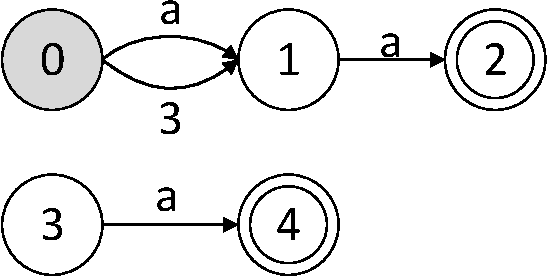
\includegraphics[width=4cm]{pictures/automatonForG0.pdf}
        \caption{Automaton for $\Gamma_{0}$}
        \label{fig:automatonForG0}
    \end{minipage}
\end{figure}

\begin{figure}
    \centering
    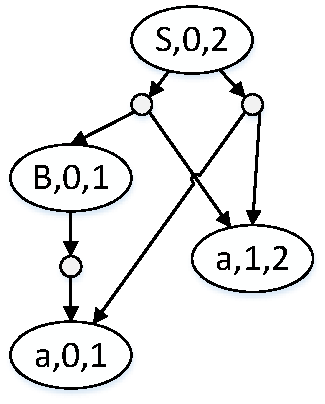
\includegraphics[width=4cm]{pictures/SPPFforG0.pdf}
    \caption{SPPF for input "aa"}
    \label{fig:SPPF}
\end{figure}


State 1 can be matched with two grammar slots: $S ::= (a \cdot a)|(b$ $a)$ and $S ::= (a$ $a)|(b \cdot a)$. 
But SPPF represents WHAT???




\textbf{function} getNodeT$(x,i)$ does not change

We defined function \textbf{getNodes} which can construct two nodes: intermediate and nonterminal (at least one of them, at most both).
It uses modified function \textbf{getNodeP} that takes additional argument: state or nonterminal name. Symbol in returned SPPF node will be this argument's value.
\begin{algorithmic}
\Function{getNodes}{$S, A, w, z$}
    \If{($S$ is final state)}
        \State $x \gets \textbf{getNodeP}(S, A, w, z)$
    \Else
        \State $x \gets \$ $
    \EndIf
    %\Statex
    %\If{$S.outedges = \varnothing$}
    %    \State $y \gets \$$
    %\Else
        \If{$(w = \$) \&$ not ($z$ is nonterminal node and it's extents are equal)}
            \State $y \gets z$
        \Else
            \State $y \gets \textbf{getNodeP}(S, S, w, z)$
        \EndIf
    %\EndIf
    
    \State \Return{$(y,x)$}
\EndFunction   
\end{algorithmic}
\begin{algorithmic}
\Function{getNodeP}{$S, L, w, z$}
    \State $(\underline{\hspace{0.25cm}}, k, i) \gets z$
    
    \If{($w \neq \$$)}
        \State $(\underline{\hspace{0.25cm}}, j, k) \gets w$
    
        \State $y \gets$ find or create SPPF node labelled $(L, j, i)$  
    
        \If{($\nexists$ child of $y$ labelled $(S, k)$)}
            \State $y\prime \gets \textbf{new}$ $packedNode(S, k)$
            \State $y\prime.addLeftChild(w)$
            \State $y\prime.addRightChild(z)$
            \State $y.addChild(y\prime)$
        \EndIf
    
    \Else
        \State $y \gets$ find or create SPPF node labelled $(L, k, i)$ 
        \If{($\nexists$ child of $y$ labelled $(S, k)$)}
            \State $y\prime \gets \textbf{new}$ $packedNode(S, k)$
            \State $y\prime.addRightChild(z)$
            \State $y.addChild(y\prime)$
        \EndIf
    \EndIf
    \State \Return{$y$}
\EndFunction
\end{algorithmic}



\section{Evaluation}

Left factorization vs EBNF

Small demo example (message to Scott)

\begin{figure}[h]
$$
\begin{array}{crcl}
& \mbox{\texttt{ S }} &::=& \mbox{\texttt{ A A A A A A | A a A A A A }} \\
& \mbox{\texttt{ A }} & ::=& \mbox{\texttt{ S A | a A | a}}\\
\end{array}
$$
\caption{Grammar $G_0$.}
\label{testGrammar}
\end{figure}

We have compared our parsers built on factorized grammar and on minimized FSA.
Grammar $G_0$(fig.~\ref{testGrammar}) was used for the tests.

Description of grammar: long ``common tail'' which is not unified with factorization.

FSA built for this grammar presented on fig.~\ref{dfa}.

\begin{wrapfigure}{R}{0.2\textwidth}
\centering
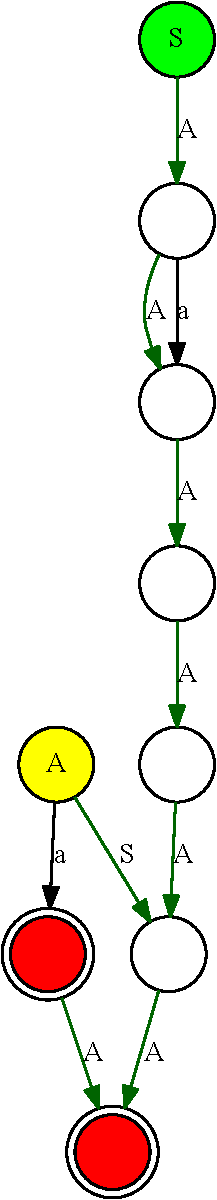
\includegraphics[width=0.15\textwidth]{pictures/minimizedDFA.pdf}
\caption{\label{dfa}Minimized automaton for grammar $G_0$}
\end{wrapfigure}

Description of input. 
Short info about PC.

Note: SPPF construction was disabled while testing.

\begin{table}[h]
\begin{center}
  \begin{tabular}{ | l | l | l | l | l | l | l | l | l | }
\hline
    Length & \multicolumn{2}{ c| }{Time, seconds} & \multicolumn{2}{ c| }{Descriptors} & \multicolumn{2}{ c| }{GSS Nodes} & \multicolumn{2}{ c| }{GSS Edges} \\ \hline
     & factorized & minimized & factorized & minimized & factorized & minimized & factorized & minimized \\ \hline
    100 & 0.206 & 0.127 & 52790 & 38530 & 200 & 200 & 42794 & 28534 \\ \hline
    200 & 1.909 & 1.54 & 215540 & 157030 & 400 & 400 & 175544 & 117034 \\ \hline
    300 & 8.844 & 7.125 & 488290 & 355530 & 600 & 600 & 398294 & 265534 \\ \hline
    400 & 25.876 & 21.707 & 871040 & 634030 & 800 & 800 & 711044 & 474034 \\ \hline
    500 & 60.617 & 51.245 & 1363790 & 992530 & 1000 & 1000 & 1113794 & 742534 \\ \hline
    1000 & 842.779 & 768.853 & 5477540 & 3985030 & 2000 & 2000 & 4477544 & 2985034 \\ \hline
     & \multicolumn{2}{ c| }{Average gain: 19$\%$} & \multicolumn{2}{ c| }{Average gain: 27$\%$} & \multicolumn{2}{ c| }{Average gain: 0$\%$} & \multicolumn{2}{ c| }{Average gain: 33$\%$} \\ \hline
\end{tabular}
\end{center}
\caption{Experiments results.}
\label{expTable}
\end{table}

Table~\ref{expTable} shows that in general minimized version works $19\%$ faster, uses $27\%$ less descriptors and $33\%$ less GSS edges.
Also we use this FSA approach in metagenomic assemblies parsing and it gives us visible performance increase. Furthermore we can use EBNF constructions without any conversion.

A bit more discussion on evaluation.


Examples of SPPF.
May be some nontrivial cases: s -> a* a* and so on


\section{Conclusion and Future Work}

Described allgorithm implemented in F\# as part of the YaccConstructor project.
Source code available here:\url{!!!}.

Proposed modification can not only increase performance, but also decrease memory usage. 
It is critical for big input processing.
For example, Anastasia Ragozina in her master's thesis~\cite{!!!} shows that GLL can be used for graph parsing.  
In some areas graphs can be really huge: assemblies in bioinfomatics ($10^8$...).
Proposed modification can improve performance not only in case of classical parsing, but in graph parsing too. 
We perform some tests that shows performance increasing in metagenomic analysis, but full integration with graph parsing and formal description is required.

One of way to specify any useful manipulations on derivation tree (or semantic of language) is an attributed grammars~\cite{!!!}.
YARD supports it but our algorithm is not.
So, attributed grammar and semantic calculation is a future work.


\bibliographystyle{abbrv}
\bibliography{bibliography}
\section{Dataset description}\label{section:dataset}

In our evaluation we use dataset which contains the following parts.
{\setlength{\tabcolsep}{0.4em}
	\begin{table}[h]
		\caption{RDFs properties}
		\label{tbl:propRDF}
		\rowcolors{2}{}{lightgray}
		\begin{tabular}{| l | c | c | c | c |}
			\hline
			Name                  & \#V    & \#E     & \#type &\#subClassOf \\
			\hline
			\hline
			atom-primitive				& 291		& 685		& 138	& 122	\\
			univ-bench					& 179		& 413		& 84		& 36		\\
			travel						& 131		& 397		& 90		& 30		\\
			skos							& 144		& 323		& 70		& 1		\\
			people\_pets					& 337		& 834		& 161	& 33		\\
			generations					& 129		& 351		& 78		& 0		\\
			foaf							& 256		& 815		& 174	& 10		\\
			biomed-mesure-prim   	    & 341		& 711		& 130	& 122	\\
			funding						& 778		& 1480		& 304	& 90               \\
			pizza						& 671		& 2604		& 365	& 259              \\
			wine							& 733		& 2450		& 485	& 126              \\
			core							& 1323		& 8684		& 1412	& 178              \\
			pathways						& 6238		& 37196		& 3118 	& 3117             \\
			go-hierarchy					& 45007		& 1960436	& 0		& 490109           \\
			enzyme						& 48815		& 219390		& 14989	& 8163             \\
			eclass\_514en				& 239111		& 1047454	& 72517	& 90962            \\
			go							& 272770		& 1068622	& 58483	& 90512            \\
			\hline
		\end{tabular}
	\end{table}
}

{\setlength{\tabcolsep}{0.4em}
\begin{table*}[h]
\caption{RDFs query $G_2$ (time is measured in seconds and memory is measured in megabytes)}
\label{tbl:tableRDFQ2}
\rowcolors{3}{}{lightgray}
\begin{tabular}{| l | r  r | r  r | r  r | r  r | r  r |}
    \hline

    \multirow{3}{*}{Name}   &   \multicolumn{6}{|c|}{Relational semantics index}	&	\multicolumn{4}{|c|}{Single path semantics index} \\
    \cline{2-11}
    &	\multicolumn{2}{|c|}{RG\_CPU\textsubscript{rel}}	&	\multicolumn{2}{|c|}{RG\_CUSP\textsubscript{rel}}	&	\multicolumn{2}{|c|}{RG\_SPARSE\textsubscript{rel}} &	\multicolumn{2}{|c|}{RG\_CPU\textsubscript{path}}	&	\multicolumn{2}{|c|}{RG\_SPARSE\textsubscript{path}}	 \\
    \cline{2-11}
    &   Time & Mem &  Time     & Mem & Time     & Mem  &  Time     & Mem & Time     & Mem \\
    \hline
    \hline
    atom-primitive          & 0.001 & 0.3  & 0.001 & 0.1 & 0.002 & 0.1   & 0.001 & 0.3  & 0.002 & 0.1   \\
biomedical-mesure-primitive & 0.002 & 0.1  & 0.014 & 2.0   & 0.009 & 0.1   & 0.006 & 0.1  & 0.012 & 0.1   \\
core                        & 0.001 & 0.3  & 0.006 & 0.1 & 0.004 & 0.1   & 0.003 & 0.3  & 0.005 & 0.1   \\
eclass\_514en               & 0.035 & 6.5  & 0.020 & 16.0  & 0.100   & 12.0    & 0.123 & 17.7 & 0.127 & 18.0    \\
enzyme                      & 0.006 & 3.9  & 0.006 & 0.6 & 0.010  & 0.1   & 0.012 & 5.3  & 0.008 & 0.4   \\
foaf                        & 0.001 & 0.1  & 0.004 & 0.1 & 0.002 & 0.1   & 0.001 & 0.1  & 0.003 & 0.1   \\
funding                     & 0.002 & 0.1  & 0.015 & 0.4 & 0.007 & 0.1   & 0.009 & 0.1  & 0.008 & 0.1   \\
generations                 & 0.001 & 0.1  & 0.001 & 0.1 & 0.001 & 0.1   & 0.001 & 0.1  & 0.001 & 0.1   \\
go-hierarchy                & 0.095 & 17.8 & 0.253 & 528.0 & 0.175 & 130.4 & 0.884 & 88.8 & 0.306 & 138.8 \\
go                          & 0.306 & 25.8 & 0.240 & 84.0  & 0.181 & 25.4  & 0.918 & 78.1 & 0.219 & 34.2  \\
pathways                    & 0.005 & 0.2  & 0.005 & 0.4 & 0.004 & 0.1   & 0.017 & 0.5  & 0.003 & 0.1   \\
people\_pets                & 0.001 & 0.1  & 0.007 & 0.1 & 0.004 & 0.1   & 0.001 & 0.1  & 0.005 & 0.1   \\
pizza                       & 0.002 & 0.3  & 0.012 & 0.2 & 0.008 & 0.1   & 0.010  & 0.3  & 0.009 & 0.1   \\
skos                        & 0.001 & 0.1  & 0.001 & 0.1 & 0.001 & 0.1   & 0.001 & 0.1  & 0.002 & 0.1   \\
travel                      & 0.001 & 0.1  & 0.007 & 0.1 & 0.005 & 0.1   & 0.001 & 0.1  & 0.005 & 0.1   \\
univ-bench                  & 0.001 & 0.1  & 0.007 & 0.1 & 0.005 & 0.1   & 0.001 & 0.1  & 0.005 & 0.1   \\
wine                        & 0.001 & 0.3  & 0.006 & 0.1 & 0.004 & 0.1   & 0.002 & 0.3  & 0.004 & 0.1  \\
    \hline
  \end{tabular}
\end{table*}
}

\begin{itemize}
\item The real-world data RDFs provided in CFPQ\_Data dataset\footnote{CFPQ\_Data dataset GitHub repository: \url{https://github.com/JetBrains-Research/CFPQ_Data}. Access date: 12.11.2019.} from~\cite{Mishin:2019:ECP:3327964.3328503}.
\item Geospecies (RDF which contains information about biological hierrarchy\footnote{The Geospecies RDF: \url{https://old.datahub.io/dataset/geospecies}. Access date: 12.11.2019.} and same-generation query over \textit{broaderTransitive} relation) is provided in~\cite{Kuijpers:2019:ESC:3335783.3335791} and integrated in our evaluation with CFPQ\_Data.
\item It was shown in~\cite{Mishin:2019:ECP:3327964.3328503} that matrix-based algorithm is performant enough to handle bigger RDFs than those used in the initial datasets, such as~\cite{RDF}.
So, we add several big RDFs to CFPQ\_Data and use them in our evaluation.
New RDFs: \textit{go-hierarchy, go, enzime, core, pathways} are from UniProt database\footnote{Protein sequences data base: \url{https://www.uniprot.org/}. RDFs with data are avalable here: \url{ftp://ftp.uniprot.org/pub/databases/uniprot/current_release/rdf}. Access date: 12.11.2019}, and \textit{eclass-514en} is from eClassOWL project\footnote{eClassOWL project: \url{http://www.heppnetz.de/projects/eclassowl/}. eclass-514en file is available here: \url{http://www.ebusiness-unibw.org/ontologies/eclass/5.1.4/eclass_514en.owl}. Access date: 12.11.2019.}.
\end{itemize}

The properties of the RDFs from the dataset are given in table \ref{tbl:propRDF}. 
Geospecies RDF contains 450609 vertices, 2311461 edges, and 20867 edges labeled by \textit{broaderTransitive}.
Note that while the number of edges labeled by \textit{broaderTransitive} is equal to provided in~\cite{Kuijpers:2019:ESC:3335783.3335791}, the total number of vertices and edges is bigger. It is because we naively convert each triple from RDF to edge in the graph, while J. Kuijpers et al. use special \textit{neosemantics}\footnote{Neosemantix is an RDF processing plugin for Neo4j. Web page: \url{https://neo4j.com/labs/nsmtx-rdf/}. Access date: 30.03.2020.} plugin which can, for example, handling multivalued properties accurately.  

The variants of the \textit{same-generation query}~\cite{FndDB} are used in almost all cases because it is an important example of real-world queries that are context-free but not regular.
So, variations of the same generation query are used in our evaluation.
All queries are added to the CFPQ\_Data dataset.

We use two queries over \textit{subClassOf} and \textit{type} relations.
The first query is the grammar $G_1$:
\[
 \begin{array}{lcl}
   s  \rightarrow \textit{subClassOf}^{\ -1} \ s \ \textit{subClassOf}   & \quad & s  \rightarrow \textit{type}^{\ -1} \ s \ \textit{type}     \\
   s  \rightarrow \textit{subClassOf}^{\ -1} \ \textit{subClassOf}       & \quad & s  \rightarrow  \textit{type}^{\ -1}  \ \textit{type}

 \end{array}
 \]
The second one is the grammar $G_2$: \[s \rightarrow \textit{subClassOf}^{\ -1} \ s \ \textit{subClassOf} \mid \textit{subClassOf}\]

For geospecies we use same-generation query \textit{geo} from the original paper~\cite{Kuijpers:2019:ESC:3335783.3335791}: \[s \rightarrow \textit{broaderTransitive} \ s \ \textit{broaderTransitive}^{\ -1} \]
\[s \rightarrow \textit{broaderTransitive}  \ \textit{broaderTransitive}^{\ -1} \]


\section{Evaluation Details}

Results for RDFs querying with $G_2$ grammar are presented in table~\ref{tbl:tableRDFQ2}.
We can see, that for small graphs time for both relational and single-path querying are similar for CPU and GPGPU versions, but for bigger graphs (\textit{go} and \textit{go-hierarchy}, for example) GPUPU version is more performant than CPU one.

\balance


\end{document}
